\documentclass[conference]{IEEEtran}
\usepackage[T1]{fontenc}
\usepackage{amsmath,amssymb,graphicx,booktabs,array,url}
\usepackage[hidelinks]{hyperref}
\usepackage{algorithm,algpseudocode}
\usepackage{microtype}
\graphicspath{{../figures/}}
\newcommand{\taumax}{\tau_{\max}}
\newcommand{\repo}{\url{https://github.com/kaustubh-dot/delayed-gradient-cpu-mlp}}
\title{Delayed Gradients in CPU-Based Neural Network Training:\\An Operating Systems Study of Bounded Staleness}
\author{\IEEEauthorblockN{Kaustubh Upadhya, Dhruv Pekhale, Jeet Mahajan, Tejas Tandon}
\IEEEauthorblockA{Indian Institute of Information Technology, Sri City\\Operating Systems Course Project}}
\begin{document}
\maketitle
\begin{abstract}
Neural-network dependencies can leave worker threads waiting even when a program uses multiple cores. We study a two-worker CPU runtime that allows genuine backpropagated gradients to arrive after the hidden layer has changed. Each layer has one owner thread, workers exchange messages through bounded queues, and the hidden owner applies a gradient only when its model-version age is within a configured limit. The workload is a 784-32-10 multilayer perceptron trained on 5,000 MNIST examples per epoch and evaluated on 1,000 test examples. Nine supplied five-epoch runs show an intermediate delay bound of four giving an observed speed-quality compromise: mean training time is 20.52 seconds versus 28.28 seconds sequentially. Because the original source and build metadata were unavailable, we also construct a documented reference implementation and execute 24 fresh runs. These runs retain the acceptance-versus-learning tradeoff but do not reproduce a speedup over optimized sequential training. Delay four averages 0.819 seconds versus 0.758 seconds sequentially, although it is substantially faster than the synchronous worker mode. The study separates synchronization savings from computation skipped by gradient rejection, explains ownership and bounded-buffer safety, and treats time to an accuracy target as a necessary companion to throughput. The evidence supports a workload-specific systems tradeoff, not a universal delay bound or CPU speedup.
\end{abstract}
\begin{IEEEkeywords}
delayed gradients, bounded staleness, operating systems, producer-consumer queues, model parallelism, CPU training
\end{IEEEkeywords}

\section{Introduction}
The question behind this project is: how much synchronization waiting can CPU workers remove while keeping neural-network training useful? A straightforward division of a network into layers gives different threads different parameter arrays. It does not remove the data dependencies between those arrays. A hidden layer produces activations needed by the output layer; the output layer produces the error signal needed to update the hidden layer. If only one example may occupy the system, the two threads repeatedly hand control to one another. The program is concurrent, but its useful arithmetic remains mostly serial.

Allowing several examples in flight changes the schedule. The hidden worker can compute another forward pass before the previous error signal returns. By then, earlier gradients may have changed its parameters. The arriving signal is still produced by backpropagation, but it refers to an older hidden-layer version. This is the delayed-gradient setting. Its purpose is to relax temporal coordination while retaining an explicit account of the age of information.

The project uses a small CPU multilayer perceptron (MLP) so that the runtime can be understood without an accelerator framework. The hidden layer has 784 inputs and 32 ReLU units; the output layer has ten logits. Worker 0 owns the hidden parameters and Worker 1 owns the output parameters. A coordinator bounds the number of submitted examples that have not completed. Messages carry an example identifier and a hidden-layer origin version. Worker 0 accepts or discards each returning gradient according to a user-selected maximum age. The policy does not undo the output update when it discards a hidden gradient.

This last detail matters for performance analysis. Discarding a gradient avoids the hidden weight update, which touches a much larger matrix than the output layer does. A shorter run can therefore reflect less arithmetic as well as more overlap. It is misleading to describe every elapsed-time reduction as synchronization removed by parallelism. The completed-example count also remains high when the hidden layer receives few updates. Training quality and useful update counts must accompany throughput.

Our evidence has two distinct origins. The supplied project artifacts contain nine five-epoch runs, a separate pair of worker-instrumented runs, a workbook, and design guides. They describe an existing prototype, but its source and original hardware/compiler settings were not supplied. We preserve those observations and analyze them as historical evidence. We then implement the described ownership and age policy in a new C++17 reference runtime, verify its mathematical and concurrency contracts, and collect an independent sweep with recorded provenance. We do not present the new source as recovered historical source or treat new runs as repetitions of the old executable.

The contributions are the explicit runtime design, its safety and liveness reasoning, a traceable analysis of the supplied measurements, and a reproducible reference study. The work adapts established delayed-gradient ideas rather than claiming a new optimization algorithm. Its operating-systems content lies in ownership, message lifetime, mutex/condition-variable coordination, finite buffers, work admission, stage imbalance, and measurement scope.

The paper follows the chosen delayed-gradient direction. Other approaches considered during the initial project survey appear only as design context. We first connect the design to primary literature, then specify its mathematics and runtime, and finally compare the two evidence sets. The public repository contains the source, raw logs, derived data, figures, report source, and reproduction commands: \repo.

\section{Literature and design context}
\subsection{Asynchronous optimization and bounded consistency}
HOGWILD! allows processors to update shared parameters without locking and analyzes conditions under which sparse update conflicts remain manageable \cite{hogwild}. It establishes a useful historical motivation for avoiding coordination on every update. Our design has different memory semantics: dense parameter arrays have one writer each, and communication uses mutex-protected queues. We neither implement lock-free shared writes nor inherit sparse-conflict guarantees for this dense MLP.

Stale synchronous parallel (SSP) computation permits bounded differences between worker progress clocks and forces faster workers to wait when the limit is exceeded \cite{ssp}. This separates strict synchronization from unconstrained asynchrony. Our age limit is related in spirit but operates at a different point. It tests a returned hidden gradient against the current hidden version and may discard it. It does not enforce the SSP parameter-server consistency model or bound a gap between independent worker clocks. A worker-progress clock, a parameter version, and a wall-clock delay are distinct quantities.

\subsection{Decoupling backpropagation with real delayed signals}
Huo et al. introduce decoupled parallel backpropagation using delayed gradients and establish convergence to critical points for their stochastic methods under the paper's assumptions \cite{ddg}. Their experiments use deeper convolutional networks and a different execution setting. We borrow the idea that backward information can be temporally delayed. Our two-layer CPU implementation, owner-thread rule, and age-based rejection policy are engineering choices for this course project. The published theorem does not by itself prove convergence of our runtime.

Features Replay addresses the memory and accuracy costs of decoupling through a parallel-objective formulation and replay of intermediate features \cite{replay}. It shows that retaining information from earlier execution is part of the algorithm, not merely a buffer-management detail. Our runtime retains each in-flight example's hidden activation and access to its input. It does not implement the Features Replay objective or repeatedly train from a replay buffer. The cache exists to preserve the forward derivative information required when a real gradient returns.

Fully Decoupled Neural Network Learning Using Delayed Gradients (FDG) seeks to break forward, backward, and update locking, and introduces gradient shrinking to reduce stale-gradient effects \cite{fdg}. Its published journal version has four authors and appears in the 2022 volume of IEEE Transactions on Neural Networks and Learning Systems. Our pipeline still requires an upstream activation before output computation. It should not be called a fully decoupled implementation of FDG. We use a binary age gate rather than the paper's gradient-shrinking procedure.

Diversely Stale Parameters (DSP) introduces layer-wise staleness and studies model-parallel training with unequal device speeds \cite{dsp}. That work is especially relevant to the distinction between delay at different modules and a single global training timestamp. Our hidden age counter measures only accepted hidden updates since an activation was produced. It does not measure the age of every parameter used to produce the downstream derivative, and it is not a full implementation of DSP.

Peng et al. combine recomputation with weight prediction in DTRP to address retained-state memory costs and the additional delay caused by recomputation \cite{dtrp}. This places two possible strategies in context: store the forward information until the gradient arrives, or recompute it later while accounting for changed weights. Our small network uses storage. It performs no weight prediction, batch compensation, or gradient correction. This simple choice makes the runtime easier to inspect, but it would need reconsideration for deep networks with large activation tensors.

\subsection{Recent work and the limits of analogy}
Ringmaster ASGD selectively ignores sufficiently stale gradients and proves time-complexity results under heterogeneous, time-varying worker computation \cite{ringmaster}. Its mathematical setting uses workers computing stochastic gradients of a common optimization objective. Our workers own different layers and exchange partial derivatives. The shared use of rejection does not make the methods equivalent. In particular, our age threshold is chosen as a small experimental control, not from Ringmaster's theoretical rule.

The 2026 dissertation \cite{recent2026} develops this asynchronous optimization line across homogeneous and heterogeneous data. It provides recent context through the literature search date of October 8, 2026, but we identify it as a dissertation rather than a new peer-reviewed conference result. The broader lesson for this project is to evaluate progress in elapsed time while stating the computation and delay assumptions. None of these references establishes that a delay of four is optimal for a two-stage CPU MLP.

\subsection{Alternatives considered in the initial survey}
Pipeline parallelism schedules micro-batches across stages to hide dependencies; GPipe provides an established example \cite{gpipe}. Dependencies remain, and stage balance, bubbles, and activation storage affect efficiency. Synthetic gradients instead estimate a missing downstream gradient using a learned model, as in decoupled neural interfaces \cite{synthetic}. Local learning substitutes a local objective. Both alter the learning signal and introduce questions beyond its age. Local SGD gives each worker a complete model and periodically averages replicas \cite{local}; its principal tradeoff is communication frequency versus replica drift.

These alternatives target different forms of coordination. The selected delayed-gradient approach keeps genuine backpropagation and one partitioned model, so the effect of stale information can be studied directly through version counters. Table~\ref{tab:space} summarizes the distinction. We do not benchmark the alternatives; the supplied artifacts and fresh experiments concern delayed gradients only.

\begin{table}[t]
\caption{Design-space context; alternatives are not implemented here.}\label{tab:space}
\centering\small
\begin{tabular}{p{.24\columnwidth}p{.66\columnwidth}}
\toprule Approach & Coordination decision \\\midrule
Delayed gradients & Use an older real derivative; track or limit its age.\\
Pipeline & Schedule another ready micro-batch while dependencies remain.\\
Synthetic/local & Predict the downstream signal or replace it with a local loss.\\
Local SGD & Train full private replicas between averaging points.\\\bottomrule
\end{tabular}
\end{table}

\section{Mathematical model and gradient semantics}
\subsection{The learning task}
MNIST is a handwritten-digit benchmark with 28 by 28 grayscale images \cite{mnist}. We normalize byte intensities to $[0,1]$ and flatten each image to $x\in\mathbb{R}^{784}$. The model computes
\begin{align}
 a_0 &= W_0x+b_0, & h&=\operatorname{ReLU}(a_0),\\
 z &= W_1h+b_1, & p_k&=\frac{\exp(z_k)}{\sum_j\exp(z_j)},\\
 \ell(x,y)&=-\log p_y.\label{eq:loss}
\end{align}
Here $W_0\in\mathbb{R}^{32\times784}$ and $W_1\in\mathbb{R}^{10\times32}$. There are 25,450 trainable scalars, including 42 biases. The model is deliberately small. Its purpose is to expose a scheduling tradeoff rather than compete with MNIST classification systems.

For one example, the output derivative is $\delta_1=p-e_y$. Before updating $W_1$, the output owner computes
\begin{align}
 d_h&=W_1^\top\delta_1,\\
 \delta_0&=d_h\odot\mathbf{1}[a_0>0],\\
 \nabla W_1&=\delta_1h^\top, & \nabla W_0&=\delta_0x^\top.
\end{align}
Bias derivatives are the corresponding local deltas. The reference implementation computes the softmax loss by subtracting the maximum logit and using the log-sum-exp expression. This avoids overflow without changing the derivative. It computes $d_h$ from the pre-update output weights; otherwise the returned signal would not match the output computation used for that example.

\subsection{Versions and the acceptance rule}
Let $v_0$ be the hidden layer's accepted-update count. When Worker 0 produces $h$ for an example, it attaches origin version $o=v_0$. When the derivative returns, its age is
\begin{equation}
 a=v_0-o.\label{eq:age}
\end{equation}
An accepted gradient increments $v_0$ by one; a rejected gradient leaves it unchanged. Thus age counts parameter changes, not examples submitted, output updates, queue operations, or elapsed milliseconds. The policy is
\begin{equation}
 \theta_0\leftarrow\theta_0-\eta g_0\quad\text{if }a\leq\taumax.\label{eq:gate}
\end{equation}
Every processed activation updates the output layer whether or not its hidden gradient later passes this test. The decision is local to Worker 0, which can compare and update the version without an atomic parameter operation.

The familiar delayed-SGD equation $\theta_{t+1}=\theta_t-\eta g(\theta_{t-a})$ is useful intuition but is not an exact description of this modular runtime. Hidden activations come from $\theta_0^o$, while the output computation uses $\theta_1^s$ when Worker 1 processes them. The returned hidden derivative is a genuine partial derivative for the pair $(\theta_0^o,\theta_1^s)$, provided the origin forward mask is retained. That pair need not have existed as a simultaneously observed complete model. A hidden age limit bounds the version difference of one module; it does not enforce a globally consistent parameter snapshot.

\begin{figure}[t]
\centering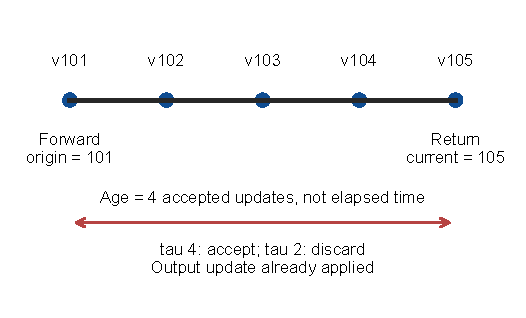
\includegraphics[width=\columnwidth]{staleness.pdf}
\caption{A conceptual version trace. The four intervening events are accepted hidden updates. This illustration is not a measured scheduling timeline.}\label{fig:age}
\end{figure}

\subsection{Why cached forward information is necessary}
The ReLU derivative must refer to the forward pass that produced the activation. If Worker 0 recomputed the mask using its newest weights, the product of the old downstream signal and a new mask would generally not be the derivative of the original example computation. We cache $h$, so its positive entries identify the origin mask. The input is immutable and remains accessible until completion. Biases and weights are updated only after the age test.

This retention policy preserves the meaning of an accepted gradient without keeping a full hidden-weight snapshot per example. For this dense layer, the weight gradient can be formed from the cached input and delta. The architecture therefore needs the input and mask, not a separate 784 by 32 matrix for every version. This is a property of the chosen layer and computation; deeper networks may need different saved tensors.

\section{Runtime architecture and operating-systems design}
\subsection{Ownership and message flow}
Figure~\ref{fig:architecture} shows the reference runtime. It uses two persistent C++17 worker threads and a coordinator on the calling thread. Worker 0 alone writes $W_0,b_0,v_0$ and its pending-example cache. Worker 1 alone writes $W_1,b_1$. The coordinator submits immutable example indices and collects results. Ownership concerns mutable parameter storage; it does not imply that every model read must run on the owner. Evaluation reads the model only after an epoch drain establishes quiescence.

\begin{figure*}[t]
\centering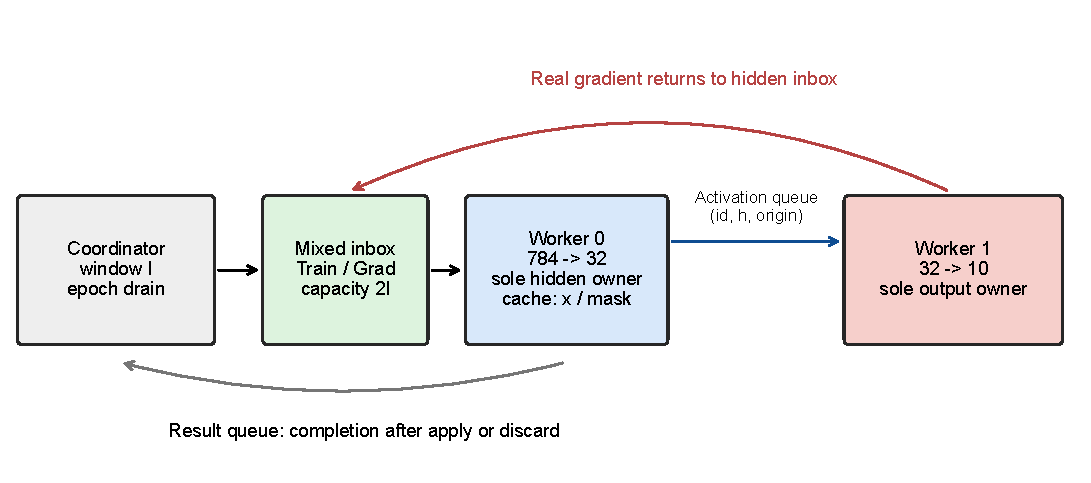
\includegraphics[width=.96\textwidth]{architecture.pdf}
\caption{Reference runtime. Work admission is bounded by $I$. Queue capacity is $2I$ in the new implementation; the original capacity is unknown. The hidden inbox serializes forward tasks and returning gradients on the same owner.}\label{fig:architecture}
\end{figure*}

There are three queues. The mixed hidden inbox accepts training messages from the coordinator and gradient messages from Worker 1. The activation queue connects the two workers. The result queue connects Worker 0 to the coordinator. A gradient shares the hidden inbox rather than entering a separate queue that would require a select operation or polling loop. A C++ variant distinguishes the two inbox message types. Table~\ref{tab:messages} records the information that crosses each edge.

The implementation's term ``batch'' in the supplied notes means one selected example in this reconstruction. No mini-batch accumulation is performed. The reference source uses an identifier for each example and stores its dataset index and hidden activation in a pending map. The identifier remains unique across epochs. The output owner consumes activations in FIFO order, forms the real derivative, applies its own update, and returns the derivative with the same identifier and origin version. Worker 0 removes the cached record after either applying or discarding the gradient, then returns a completion result.

\begin{table}[t]
\caption{Messages in the reference runtime.}\label{tab:messages}
\centering\small
\begin{tabular}{p{.26\columnwidth}p{.64\columnwidth}}
\toprule Message & Payload and purpose \\\midrule
Training & Unique ID and immutable dataset index; request hidden forward work.\\
Activation & ID, label, hidden origin, 32 doubles; request output work.\\
Gradient & ID, origin, 32 derivatives, pre-update loss; return hidden learning signal.\\
Result & ID, measured age, acceptance flag, loss; release in-flight credit.\\\bottomrule
\end{tabular}
\end{table}

\subsection{Bounded admission and finite buffers}
The coordinator maintains submitted and completed counters. It admits work only while
\begin{equation}
 n_{\mathrm{submitted}}-n_{\mathrm{completed}}<I.\label{eq:window}
\end{equation}
This invariant bounds outstanding examples and pending forward state. A completion releases one credit even if the hidden update was rejected. Bounded admission and bounded queue storage serve related but different purposes: the first limits end-to-end outstanding work; the second prevents an individual channel from growing without limit.

Queue capacity is $2I$ in the reconstruction. A FIFO deque, mutex, and two condition variables implement each channel. A push waits until the queue has room or is closed. A pop waits until the queue contains an item or is closed. Predicate-based waits handle spurious wakeups correctly. The operation changes the deque while holding the mutex, then notifies the opposite side. It releases the mutex when it returns, before any layer arithmetic begins.

Using a small arbitrary capacity in a cyclic graph can deadlock: a hidden worker might block pushing an activation while the output worker blocks returning a gradient to a full hidden inbox. Capacity must therefore be considered together with admission, message lifetime, and routing. Under the reference protocol, an outstanding example contributes at most one queued message to a given channel. With at most $I$ outstanding examples and capacity $2I$, queue exhaustion cannot form that cycle in a normal epoch. This is a conservative protocol-specific argument. It is not a claim that any three bounded queues are deadlock-free.

The queues still enforce producer-consumer waiting when empty. Their capacity is an upper bound rather than evidence that producers often block on a full queue. We record maximum occupancy and a push-admission timer in the fresh logs. That timer starts before mutex acquisition and stops when the condition-variable predicate permits progress, before deque insertion. It includes lock acquisition and any predicate wait, but not the entire push call or container mutation. A nonzero value does not alone demonstrate capacity backpressure. Actual observed occupancy must be compared with capacity.

\subsection{Safety, lifetime, and epoch drains}
Parameter safety follows from disjoint write ownership. A hidden update and a hidden forward pass execute on the same thread, so the version corresponds to the parameter state used by that forward pass. Output work also runs serially. Workers exchange copied activation and derivative arrays instead of references to mutable layer arrays. The dataset never changes while workers run. A pending record survives until its matching gradient is processed.

Evaluation begins only after every submitted example has returned a result. The output update occurs before the corresponding gradient is enqueued, and the hidden decision occurs before the result is enqueued. Mutex release/acquire operations on the queues establish the required ordering between workers and coordinator. After the coordinator drains all results, no outstanding activation can still modify either layer. Workers may be sleeping in queue pops; that does not prevent safe read-only evaluation. New training messages arrive only after evaluation finishes.

Draining also defines the epoch boundary. The system never labels a partly processed epoch as a checkpoint, and no retained activation crosses from one epoch into the next. Thread startup precedes the training timer. Test evaluation lies outside every timed training window. The reported training duration is the sum of these windows, which includes coordination, layer computation, and message transfer during training.

\subsection{Shutdown and progress}
At final completion the coordinator closes the hidden inbox. Closure wakes blocked producers and consumers. A pop may drain queued items after closure; it returns failure only when the closed queue is empty. Once Worker 0 leaves its loop, it closes the activation queue, waking Worker 1, and both threads are joined. Normal termination follows an epoch drain, so no live gradient still needs delivery when shutdown begins.

Progress requires that the OS eventually schedule each participant and that the arithmetic and queue operations terminate. No algorithm here can guarantee progress under permanent thread starvation. Under fair-enough scheduling and valid input, FIFO channels preserve each producer's message order, caches are consumed exactly once, and each admitted example produces one output update and one result. The result count conservation is a useful executable check of this argument. The implementation does not use busy waiting, opportunistic shared-weight reads, or detached worker threads.

\section{Algorithm and implementation checks}
Algorithm~\ref{alg:runtime} gives the hidden owner and coordinator policies. Worker 1 applies its output update before returning the hidden derivative, as specified above. The sequential baseline executes the same forward and derivative functions in one thread. The synchronous worker configuration sets $I=1$ and $\taumax=0$, so a new example cannot enter until the previous hidden decision completes.

\begin{algorithm}[t]
\caption{Bounded delayed-gradient training}\label{alg:runtime}
\begin{algorithmic}[1]
\State Initialize both layers and owner threads; $v_0\gets0$
\For{each epoch}
 \State Shuffle fixed training indices; $s\gets0$, $c\gets0$
 \While{$c<N$}
  \While{$s<N$ and $s-c<I$}
   \State Send training index with fresh ID; $s\gets s+1$
  \EndWhile
  \State Receive result; record loss, age, decision; $c\gets c+1$
 \EndWhile
 \State Stop epoch timer; evaluate drained model
\EndFor
\State Close hidden inbox; join workers
\Statex \textbf{Worker 0, for each mixed-inbox message:}
\If{message is training work}
 \State Compute $h$ at $v_0$; cache input index and $h$
 \State Send $(\mathrm{ID},h,y,o=v_0)$ to Worker 1
\Else
 \State Retrieve matching cache; $a\gets v_0-o$
 \If{$a\leq\taumax$}
  \State Form gradient using cached mask; update hidden layer
  \State $v_0\gets v_0+1$
 \EndIf
 \State Erase cache; send result for this ID
\EndIf
\end{algorithmic}
\end{algorithm}

The two settings $\taumax=0,I=1$ and $\taumax=0,I=8$ are not equivalent. In the first, no other hidden update can occur between an example's forward pass and its returned gradient. In the second, several forward passes may share one origin version. The first accepted gradient advances the hidden version; following gradients from that origin are then too old for the zero-age gate. The output layer nevertheless receives all their updates. This provides a direct explanation for high completed throughput with low hidden acceptance.

We verify mathematical correctness using centered finite differences on a synthetic input, sampling both weight matrices and testing every bias. The test compares numerical loss derivatives with the gradients implied by a small learning-rate update. It also checks stable loss evaluation at very large logits. These checks exercise the pre-update output derivative and cached hidden mask, rather than merely checking that the program executes.

Concurrency tests cover queue close-and-drain semantics, closed pushes, and producer/consumer calls racing with closure. Their readiness promises are set before queue entry, so they do not establish that a thread was already blocked when closure occurred. Integration tests create tiny IDX-format fixtures without downloading MNIST. Sequential and synchronous runs must match training loss, test loss, test accuracy, and a weighted parameter checksum at every checkpoint to nine decimal places. Delayed runs must conserve accepted plus discarded counts, perform one output update per example, obey the accepted-age limit, and remain within the in-flight bound. Invalid nonpositive admission settings must fail before training.

All four integration tests pass, including the executable self-test. The fresh experiment harness checks count and age invariants for every recorded epoch as well. These tests provide evidence for the intended contracts; they do not constitute an exhaustive formal proof of every possible interleaving. In particular, platform scheduling and toolchain behavior still need consideration when porting the runtime.

\section{Theoretical performance and staleness analysis}
\subsection{A service-cost model}
Let $F_0$ denote hidden forward cost, $B_0$ hidden gradient-application cost, and $U_1$ the output forward/backward/update cost. For $N$ examples, a simple sequential arithmetic model is
\begin{equation}
 T_{\mathrm{seq}}\approx N(F_0+B_0+U_1).\label{eq:seqcost}
\end{equation}
Let $r$ be the hidden acceptance fraction. A delayed run performs approximately $N$ hidden forwards and output updates but only $rN$ hidden gradient applications. Its worker service demands are
\begin{equation}
 D_0=N(F_0+rB_0),\qquad D_1=NU_1.\label{eq:demands}
\end{equation}
A lower-bound intuition is $T_{\mathrm{delay}}\gtrsim\max(D_0,D_1)$ before admission, queue, scheduling, and memory costs. Actual time also includes those overheads and startup/drain bubbles within the epoch. Equations~\ref{eq:seqcost} and~\ref{eq:demands} are a model, not fitted measurements; the supplied logs do not isolate the component costs.

The hidden matrix has 25,088 weights, while the output matrix has 320, a ratio of 78.4. Both the hidden forward and accepted hidden update traverse the larger matrix. This gives a structural reason to expect stage imbalance, but it is not an assertion that Worker 0 takes exactly 78.4 times longer. ReLU masks, memory access, loop optimization, message copies, and fixed overhead all affect elapsed service time.

If $U_1$ is small, overlapping it with hidden work can remove only a small share of total arithmetic time. By contrast, lowering $r$ can remove a substantial amount of hidden update work. That observation explains why a rejection-heavy mode can be fastest while learning least well. A fair systems interpretation therefore asks whether speed comes from overlapping comparable work, avoiding wakeup overhead, or skipping updates. The present experiment cannot uniquely attribute old timing differences to those mechanisms.

\subsection{Useful throughput and target time}
For measured training time $T$, we distinguish
\begin{equation}
 q_{\mathrm{complete}}=\frac{N}{T},\qquad
 q_{\mathrm{accepted}}=\frac{rN}{T}.\label{eq:rates}
\end{equation}
The output update rate equals $q_{\mathrm{complete}}$ in this protocol. An accepted hidden update remains a computational count, not a guarantee of equal optimization value: an old accepted gradient can affect the objective differently from a current one. Nevertheless, reporting it prevents the especially misleading case of treating rejected work as hidden-layer progress.

For target accuracy $A$, the reported target time is
\begin{equation}
 T_A=T_{e^*},\quad e^*=\min\{e:\operatorname{accuracy}_e\geq A\}.\label{eq:target}
\end{equation}
If no recorded checkpoint qualifies, $T_A$ is not reached within the experimental horizon. It is not zero or infinity as a measured value. Checkpoint-based observation leaves the exact crossing time unmeasured. It also does not guarantee that every later checkpoint remains above target. A run that reaches 90\% and later dips below it still has a first qualifying checkpoint under this definition.

\subsection{Delay bounds and their scope}
Every accepted hidden gradient has $a\leq\taumax$ by construction. A further bound in this particular FIFO runtime is $a\leq I-1$ for every returned gradient. At the example's forward pass, there are at most $I-1$ other outstanding examples. The single output owner processes activations in their forward order, and its returning gradients preserve that order in the mixed FIFO inbox. Later activations cannot have their hidden gradients applied before this example. Only earlier outstanding gradients can advance its hidden version before it returns, giving the bound.

This argument depends on FIFO ordering and one output producer. It would not automatically hold with out-of-order output execution, priorities, multiple output workers, retries, or a replay scheme. In-flight admission alone is not a general bound on age for arbitrary asynchronous systems. The fresh logs obey the bound, and all accepted ages obey their configured gate.

For $I=8$, delay limits eight and sixteen both exceed the reachable age of seven. Their acceptance policies are therefore equivalent in this reconstruction. Separate runs can still differ because thread scheduling changes the sequence of forwards relative to hidden updates. A difference between their measured accuracies cannot be attributed to one bound accepting ages that the other rejects. The supplied guides mention an earlier delay-sixteen sweep but contain no numeric measurements for it; we do not reconstruct an old value from that mention.

\subsection{A conditional optimization intuition}
For an illustrative smooth full-model objective with Lipschitz gradient constant $L$, bounded gradient norm $G$, constant step $\eta$, and $a$ intervening updates,
\begin{equation}
 \|\nabla F(\theta_t)-\nabla F(\theta_{t-a})\|
 \leq L\|\theta_t-\theta_{t-a}\|\leq L\eta Ga.
\end{equation}
This shows why delay and step size can interact: more parameter movement permits greater derivative mismatch. It is a conditional bound derived from the stated assumptions, not a convergence theorem for our implementation. ReLU has nonsmooth points; the two owners use different versions; learning rate is constant; and age-dependent rejection may change the sampled updates. We do not establish the assumptions needed to transfer a published stochastic convergence guarantee.

Rejection also changes the effective training stream. Since worker service and scheduling can depend on which ReLU units are active, acceptance need not be independent of the input. Even when the coordinator presents a fixed shuffled dataset, the hidden layer may learn from a scheduling-dependent subset. That is another reason not to equate an accepted update with an unbiased stochastic gradient at the current model.

\subsection{Memory and queue costs}
The model parameters occupy $25{,}450\times8=203{,}600$ bytes of double payload. Cached hidden activations require $32\times8=256$ bytes per pending example, plus indices, identifiers, map nodes, and allocator overhead. The immutable selected training vectors alone occupy $5{,}000\times784\times8=31{,}360{,}000$ bytes. These are calculated payload sizes, not measured resident-set sizes.

Retained forward state grows as $O(IH)$ when inputs are represented by references to immutable dataset storage, and input storage grows as $O(ND)$. Message buffers also grow with $I$ and payload width. The source avoids parameter replication per worker and full-model snapshots per version. This makes the memory behavior easy to bound for a small dense model. It does not justify a claim about peak process memory, cache miss rate, or NUMA efficiency, none of which is measured here.

\section{Experimental method and provenance}
\subsection{Controlled workload}
Both evidence sets describe five epochs, 5,000 selected training examples per epoch, 1,000 selected official test examples, learning rate 0.01, and seed 12345. In the reconstruction, the first 5,000 training records and first 1,000 test records are selected before training. The selected training indices are shuffled every epoch with a persistent seeded Mersenne Twister. Hidden weights use normal scale $\sqrt{2/784}$ and seed 12345; output weights use scale $\sqrt{1/32}$ and seed 12346; biases start at zero.

The original guides describe seeded normal initialization and shuffling, but do not provide the source, precise subset identities, loop order, numeric type, or standard-library random implementation. Identical settings on paper therefore do not guarantee identical model trajectories across the two studies. We do not merge their rows, compute a pooled timing mean, or claim the new executable reproduces original accuracy exactly.

\subsection{Evidence sets and audit}
The original epoch CSV contains 45 checkpoint rows across nine runs. Its comparison CSV contains the corresponding nine final rows. Two sequential runs and two delay-four runs are available; the other primary settings have one run each. The workbook's 45 data rows match the epoch CSV within $10^{-6}$, and every final metric and first-90\% checkpoint agrees between the two CSVs.

The timing log contains one additional delay-four run and one additional synchronous run. Both have five checkpoint rows, but they are not extra rows in the primary CSVs. Its section headings are reversed: the block headed synchronous reports $\taumax=4,I=8$, and the block headed delayed reports $\taumax=0,I=1$. The numeric fields identify the runs. We preserve the raw file byte for byte and write a corrected derived copy and extracted timing CSV. The supplied demo notes repeat the same label problem, so the repository includes a separate usable demo guide.

Fresh measurements use an Intel Core i5-12450H with 12 logical processors, Windows 11 build 26300, and MSYS2 MinGW GCC 15.2.0. The scalar C++17 executable is compiled with \texttt{-O2 -std=c++17 -pthread}; warning flags are also enabled. The experiment metadata records source and executable SHA-256 hashes, decompressed dataset hashes, commands, and timing definitions. The separate downloader verifies compressed MNIST checksums; those checks are not fields in the experiment metadata. These fresh timings refer to this executable; no BLAS library, GPU, or framework data loader is used.

\subsection{Repetitions, scheduling, and metrics}
We run three repetitions of each of eight configurations: sequential, synchronous $(0,1)$, and delayed $(0,8),(1,8),(2,8),(4,8),(8,8),(16,8)$. Within each repetition, configurations run serially in a reproducibly randomized order. Each process begins from the same initialization seed. Repetitions expose timing and asynchronous scheduling variation; they are not independent initialization seeds or new dataset samples.

Affinity is not pinned, background load is not controlled, and turbo/power-state effects are not profiled. These constraints are recorded rather than guessed. Fresh training windows are less than a few seconds, so scheduler noise and fixed overhead can affect their ratios. We report means and observed ranges, not confidence intervals or claims of statistical significance.

At each drained epoch, we record average pre-update training loss, test loss, test accuracy, cumulative training seconds, accepted and discarded hidden counts, output updates, average and maximum ages, maximum pending count, and a parameter checksum. Whole-run stderr logs record worker active paths, input-pop admission durations, queue high-water marks, and push-admission durations. The input-pop counters can include evaluation gaps across the worker lifetime, while training time excludes evaluation. Active-path intervals include the complete processing and push calls. These measurements have different denominators and must not be added into one supposed CPU budget.

\section{Analysis of supplied measurements}
\subsection{Learning curves and final quality}
Figure~\ref{fig:oldlearn} preserves the learning trajectory rather than using only final checkpoints. Means are taken only within repeated configurations; shaded bands show their observed range. Sequential and synchronous curves have identical loss and accuracy values in the supplied CSV. This supports the documented intent of a one-example handshake, although it cannot replace source inspection for the original implementation.

\begin{figure*}[t]
\centering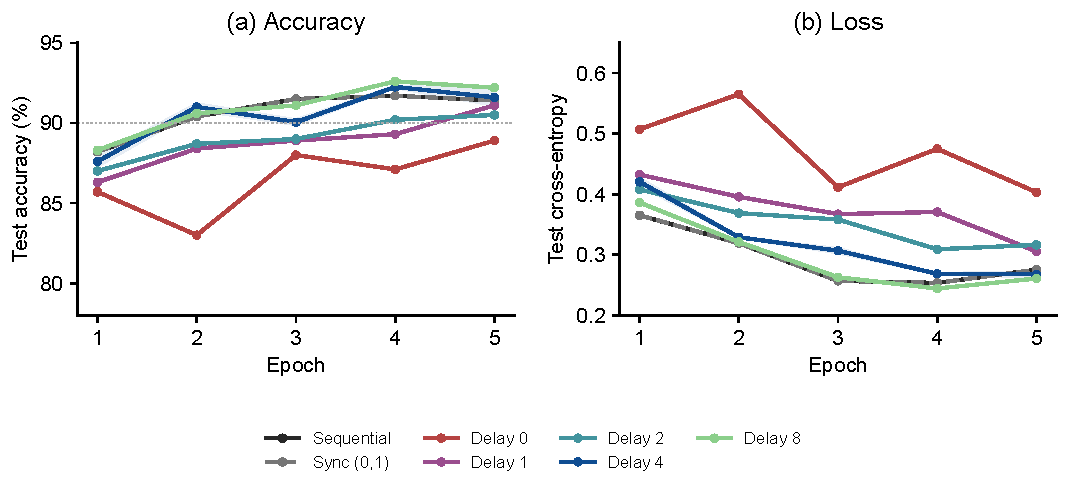
\includegraphics[width=.96\textwidth]{supplied_learning.pdf}
\caption{Supplied test curves. Sequential and synchronous curves coincide in quality. Bands show the range of the two sequential and two delay-four observations; singleton settings have no uncertainty band. The separate instrumented runs are excluded here.}\label{fig:oldlearn}
\end{figure*}

The strict asynchronous zero-age setting ends at 88.9\% after five epochs. Delay one reaches 91.1\% only at epoch five, and delay two reaches its first 90\% checkpoint at epoch four. Delay four reaches the target at epoch two in both CSV runs. Their final accuracies are 92.1\% and 91.1\%; their test-loss values are 0.263285 and 0.271865. Delay eight accepts all hidden gradients and finishes at 92.2\%. These observations do not form a monotonic relationship between delay and convergence speed.

Accuracy is also nonmonotonic within runs. The first delay-four run reaches 90.8\% at epoch two, drops to 89.9\% at epoch three, and finishes above 92\%. Training loss continues to decrease, but that does not force the test decision rate to rise at every checkpoint. Test loss measures confidence as well as classification correctness, so its ordering need not match accuracy exactly.

\subsection{Time, acceptance, and the observed compromise}
Table~\ref{tab:old} and Fig.~\ref{fig:oldtrade} summarize the primary supplied sweep. Mean sequential time is 28.279 seconds and mean delay-four time is 20.521 seconds. The ratio of those descriptive means is 1.378. Their mean first-90\% times are 11.128 and 8.267 seconds, respectively, a descriptive ratio of 1.346. The two delay-four runs are both quicker to the target than either recorded sequential run.

\begin{table}[t]
\caption{Supplied primary runs. Values are per-setting means; NR means the target was not reached. $n$ is the observed run count.}\label{tab:old}
\centering\scriptsize
\begin{tabular}{lrrrrr}\toprule
Setting & $n$ & Time (s) & Acc. (\%) & Accept (\%) & $T_{90}$ (s)\\\midrule
Sequential & 2 & 28.279 & 91.40 & 100.00 & 11.128 \\
Sync (0,1) & 1 & 28.614 & 91.40 & 100.00 & 11.536 \\
Delay 0 & 1 & 9.997 & 88.90 & 12.50 & NR \\
Delay 1 & 1 & 11.183 & 91.10 & 27.17 & 11.183 \\
Delay 2 & 1 & 15.757 & 90.50 & 47.97 & 12.710 \\
Delay 4 & 2 & 20.521 & 91.60 & 70.28 & 8.267 \\
Delay 8 & 1 & 26.584 & 92.20 & 100.00 & 10.756 \\
\bottomrule\end{tabular}

\end{table}

\begin{figure*}[t]
\centering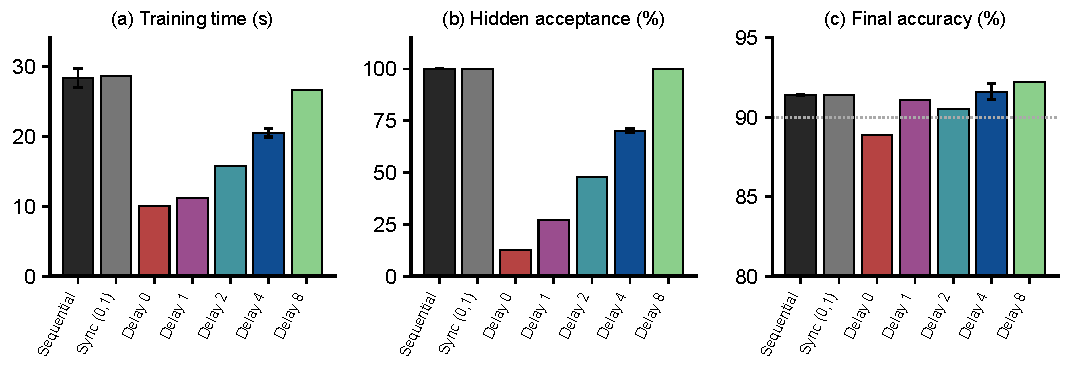
\includegraphics[width=.96\textwidth]{supplied_tradeoff.pdf}
\caption{Supplied elapsed time, hidden acceptance, and final accuracy. Error whiskers show only observed minimum and maximum for repeated settings. Accuracy uses a restricted vertical scale to show differences.}\label{fig:oldtrade}
\end{figure*}

Zero-age delayed execution is fastest at 9.997 seconds, but accepts only 12.5\% of hidden gradients. Over 25,000 completed examples, that implies 3,125 hidden updates. Its completed rate is about 2,501 examples per second, while its accepted hidden rate is about 313 updates per second. Delay four averages 70.28\% acceptance across the two primary runs. Its per-run accepted update rates are about 869 and 845 updates per second. High completed throughput at delay zero therefore does not translate into a higher accepted hidden update rate, let alone faster attainment of useful accuracy.

The synchronous run accepts all updates and reaches the same final quality as sequential training, but its 28.614-second time lies within the 26.922 to 29.635-second sequential range. The data do not establish that adding two worker threads improves this strict execution. Delay eight takes 26.584 seconds, close to the sequential observations, despite its good final accuracy. The observed delay-four compromise combines fewer hidden updates with earlier useful quality. It should not be interpreted as equal-work parallel speedup.

\subsection{Separate worker-instrumented observations}
The numeric delayed $(4,8)$ timing block reports 18.727 seconds, 63.52\% acceptance, and 91.0\% final accuracy. Its first target checkpoint is 7.472 seconds at epoch two. The synchronous $(0,1)$ block reports 28.951 seconds, full acceptance, and 91.4\% final accuracy, with target time 11.630 seconds. These are consistent with the broad historical pattern, but they remain separate observations.

\begin{figure*}[t]
\centering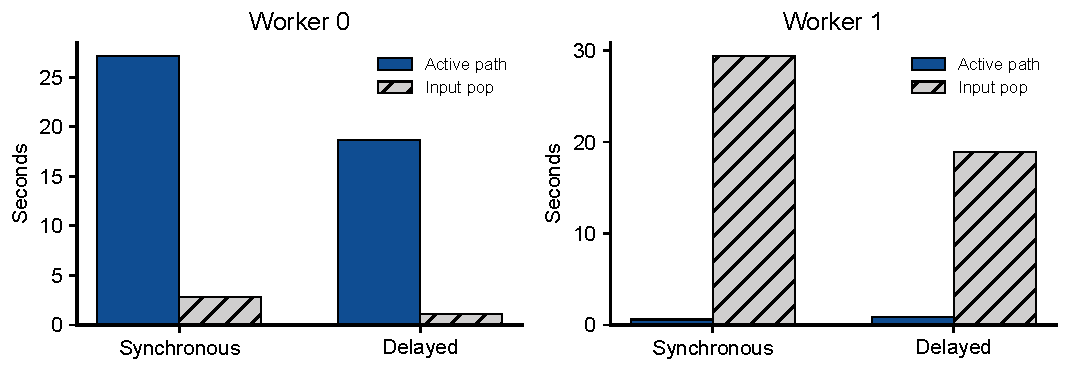
\includegraphics[width=.96\textwidth]{supplied_worker_timing.pdf}
\caption{The two supplied instrumented runs, identified by their numeric configuration. Active-path and input-pop measurements overlap across workers and include different intervals from the training timer; this is not a CPU-utilization chart.}\label{fig:wait}
\end{figure*}

Worker 0's active path is 18.690 seconds delayed versus 27.146 seconds synchronous; its input-pop duration is 1.102 versus 2.851 seconds. Worker 1's active path is only 0.817 versus 0.586 seconds, while input-pop duration is 18.966 versus 29.421 seconds. The output worker thus spends much more measured time in its input path than its arithmetic path. The small output layer and larger hidden stage give a coherent explanation for the imbalance.

These numbers do not form a partition of wall time. For example, Worker 1's synchronous input-pop duration exceeds the reported 28.951-second training duration. The supplied guide describes broader worker intervals including startup and shutdown, but original source is unavailable to verify exact boundaries. Evaluation gaps are another plausible contribution, rather than an independently established fact about that executable. Summing overlapping per-thread times or turning them into CPU utilization percentages would create a metric the logs never measured. The lower absolute delayed wait is partly associated with a shorter run; it does not establish that the output worker has become well utilized.

\section{Fresh reference experiments}
\subsection{What reproduces and what does not}
Table~\ref{tab:fresh} reports the fresh sweep, and Fig.~\ref{fig:newlearn} shows its curves. Sequential and synchronous runs have identical epoch losses, accuracies, and parameter checksums in all three repetitions. Both finish at 91.8\%. This supports the correctness of the reference one-example worker handshake. Delayed runs vary with scheduling even though initialization and data order are fixed.

\begin{table}[t]
\caption{Fresh reference sweep: three scheduling repetitions per setting, five epochs. All values are descriptive means. Targets are reached by all three runs where a value appears.}\label{tab:fresh}
\centering\scriptsize
\begin{tabular}{lrrrrr}\toprule
Setting & $n$ & Time (s) & Acc. (\%) & Accept (\%) & $T_{90}$ (s)\\\midrule
Sequential & 3 & 0.758 & 91.80 & 100.00 & 0.469 \\
Sync (0,1) & 3 & 2.558 & 91.80 & 100.00 & 1.549 \\
Delay 0 & 3 & 0.715 & 86.37 & 13.40 & NR \\
Delay 1 & 3 & 0.754 & 87.90 & 27.59 & NR \\
Delay 2 & 3 & 0.771 & 89.10 & 41.54 & NR \\
Delay 4 & 3 & 0.819 & 90.80 & 70.68 & 0.659 \\
Delay 8 & 3 & 0.851 & 91.30 & 100.00 & 0.580 \\
Delay 16 & 3 & 0.903 & 91.33 & 100.00 & 0.626 \\
\bottomrule\end{tabular}

\end{table}

\begin{figure*}[t]
\centering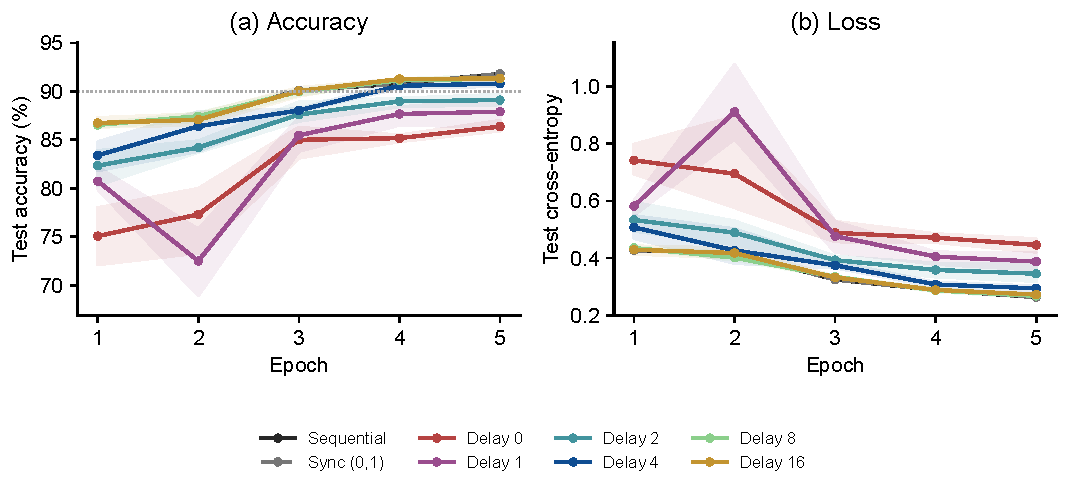
\includegraphics[width=.96\textwidth]{fresh_learning.pdf}
\caption{Fresh reference learning curves. Each mean and observed range uses three scheduling repetitions. These are a separate source/build study, not additional original-prototype runs.}\label{fig:newlearn}
\end{figure*}

The acceptance pattern is similar to the supplied one. Zero-age delayed mode accepts 13.40\% on average; delays one, two, and four accept 27.59\%, 41.54\%, and 70.68\%, respectively. Delays eight and sixteen accept every hidden gradient. The tightest settings again lose learning quality: delay zero finishes between 85.9\% and 87.0\%, delay one between 86.3\% and 89.2\%, and delay two between 88.6\% and 89.7\%. None reaches a 90\% checkpoint in its five-epoch horizon.

Delay four finishes between 90.5\% and 91.1\%, reaches the target in all three runs, and averages 90.8\% final accuracy. Delay eight finishes between 91.0\% and 91.7\%, while delay sixteen finishes between 91.0\% and 91.5\%. Full acceptance is useful for learning in this study, but it does not reproduce the exact original trajectories. The fresh initial state, subset identity, and numeric execution are documented; the original equivalents are unavailable.

\subsection{The sequential comparison changes the conclusion}
Fresh mean training times are 0.758 seconds sequentially, 2.558 seconds synchronously, and 0.819 seconds for delay four. The sequential range is 0.741 to 0.788 seconds; delay four spans 0.710 to 0.961 seconds. The ratio of mean sequential to delay-four time is about 0.926, so the delayed mode has no mean speedup over sequential execution. One delayed run is faster, but two are slower. A claim of general improvement would be unsupported.

Against the synchronous worker mode, delay four has a descriptive 3.125 ratio of mean times. This is an improvement over a fine-grained inter-thread handshake, which is expensive relative to optimized scalar arithmetic on this workload. It is not the same comparison as beating a single-thread implementation. At zero delay with one example in flight, queue locks and wakeups occur around nearly every small computational dependency. Increasing in-flight work reduces this repeated serial handoff, while rejection also removes some hidden update arithmetic.

\begin{figure*}[t]
\centering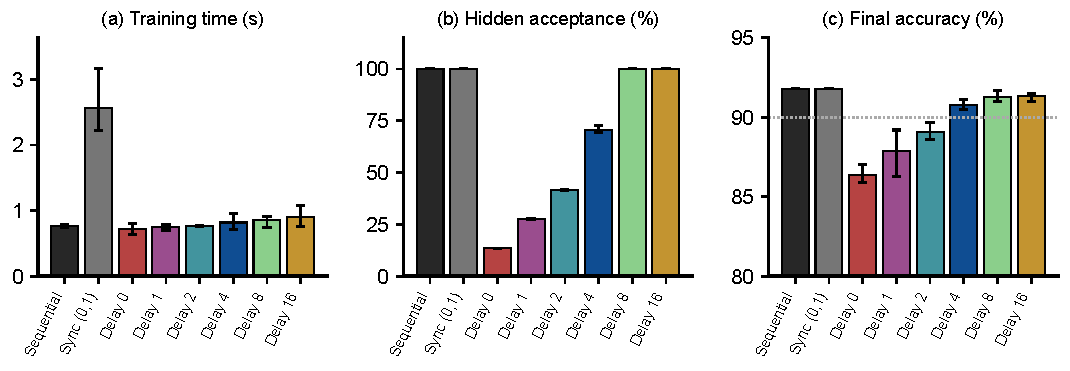
\includegraphics[width=.96\textwidth]{fresh_tradeoff.pdf}
\caption{Fresh elapsed-time and learning tradeoff. The optimized sequential baseline is competitive with every delayed mean and reaches the target sooner. Whiskers are observed ranges across three runs; they are not confidence intervals. Accuracy uses a restricted vertical scale.}\label{fig:newtrade}
\end{figure*}

The overall fresh arithmetic is much faster than the supplied measurements. We cannot attribute this roughly tens-of-seconds to subsecond change to compiler optimization alone because the original source, hardware, flags, and exact loops are unknown. The new source is scalar C++ compiled at \texttt{-O2}, with index-based immutable inputs and small copied activation arrays. Those properties explain why its provenance matters, but they do not establish a causal account of the old-new timing gap.

\subsection{Time to useful quality}
Sequential training first reaches 90\% at a mean 0.469 seconds. Delay four reaches it at 0.659 seconds, delay eight at 0.580 seconds, and delay sixteen at 0.626 seconds. The synchronous mean is 1.549 seconds. Figure~\ref{fig:targets} shows every observed delayed target point, with nonreaching settings explicitly marked. We do not substitute elapsed final time for an unachieved target.

\begin{figure*}[t]
\centering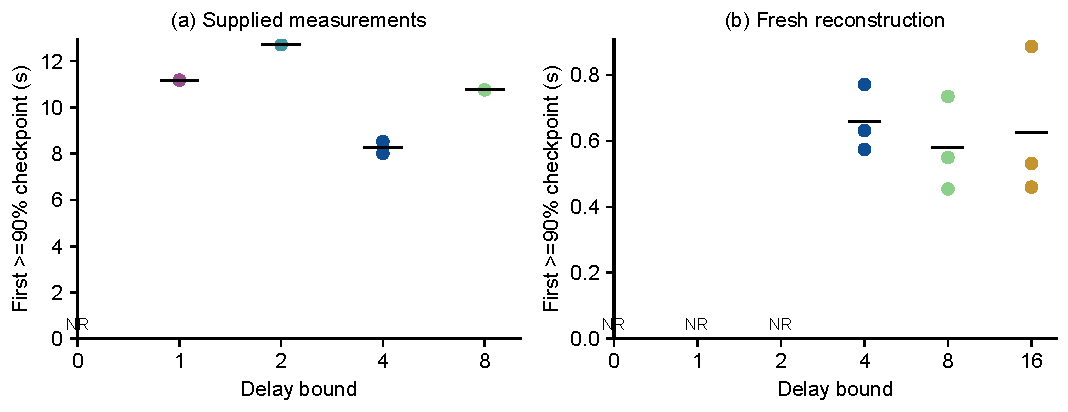
\includegraphics[width=.96\textwidth]{time_to_target.pdf}
\caption{Time to the first recorded 90\% test-accuracy checkpoint. Each dot is a run; short horizontal ticks mark the descriptive mean for reaching runs. NR means no checkpoint reached the target in five epochs. Original and fresh time scales are separate.}\label{fig:targets}
\end{figure*}

The fastest fresh completion setting, delay zero, averages 0.715 seconds but never reaches the quality threshold. This is the same methodological warning as in the supplied study, even though the actual rates differ. Delay four beats synchronous training on target time but trails sequential training. Delay eight has full acceptance and a lower mean target time than delay four, despite its longer mean five-epoch time. The ``best'' configuration depends on the chosen objective, and the fresh evidence does not select delay four as a universal winner.

\subsection{Age and instrumentation checks}
All 120 fresh epoch rows satisfy accepted plus discarded equals 5,000 and output updates equals 5,000. Every accepted age is within its configured gate; every observed age is at most seven; every maximum pending count is within the configured window. The age-eight and age-sixteen settings both accept all gradients, as the FIFO bound predicts. Their differing test curves are scheduling observations, not evidence for a meaningful acceptance-policy difference.

Across fresh repetitions, mean age over all returned gradients is 0.866, 1.615, 2.242, and 3.140 for delay limits zero, one, two, and four. The corresponding pooled mean accepted ages are 0, 0.603, 1.175, and 2.368. Their maximum observed ages are one, two, three, and five, including rejected gradients. Delays eight and sixteen have mean ages 3.511 and 3.517 and maximum age seven. In the separate supplied instrumented delay-four run, mean returned age is 3.124960, mean accepted age is 2.048111, and maximum age is five. The maximum returned age can exceed the configured gate because it includes rejected messages.

The fresh stderr logs also contain queue occupancy high-water marks and timing counters. Across the delayed runs, each channel's observed maximum occupancy is at most eight, below its capacity of sixteen. These are maximum observed occupancies, not time-weighted distributions, and they do not show full-buffer blocking in this sweep. Input-pop admission counters accumulate across the worker lifetime and can include time when the coordinator evaluates checkpoints. Like the push-admission timer, each pop timer stops after the predicate wait, before deque removal. These counters include lock acquisition and condition-variable waiting, not container mutation or the complete call. We publish them for inspection, but do not call them CPU usage, scheduler traces, or evidence of memory-bandwidth saturation.

\section{Discussion: what the operating systems experiment shows}
\subsection{Synchronization granularity matters}
The results distinguish the cost of using threads from the benefit of overlapping work. With one example in flight, workers serialize small tasks through queue operations. That provides a useful controlled baseline for inter-thread coordination, but it is a poor assumption for demonstrating CPU speedup. The reference synchronous implementation reproduces the sequential learning path while taking substantially longer, so its extra time is associated with the worker protocol rather than a different objective or missing updates.

Allowing eight examples in flight amortizes some handoff costs across ready work. The hidden worker can process several training messages while gradients are pending. Yet the output stage remains much smaller than the hidden stage, and the hidden owner's serial stream includes both forwards and accepted updates. There is no reason to expect two workers to provide a twofold gain when one stage owns most arithmetic. The design gives overlap opportunities; the partition limits their value.

The project also demonstrates that an age gate affects a system's service demand. As the gate becomes stricter, more results complete without a hidden update. Throughput can rise because the server performs less work, even if no additional arithmetic runs simultaneously. A more demanding evaluation would compare against a sequential implementation that deliberately drops the same number and identity of hidden updates. That control is not present in the current experiments, so we describe the observed modes rather than assigning all improvement to parallelism.

\subsection{Ownership simplifies reasoning, but does not erase costs}
Single-writer layer ownership removes the need for a parameter lock around every scalar update. It also gives a precise place to increment the version and make an age decision. Race avoidance follows from access discipline and message ordering, not from the mere presence of a mutex somewhere in the program. The coordinator's epoch drain is as important as worker ownership because evaluation otherwise could read weights while an owner modifies them.

Queue synchronization moves the contention boundary to message transfer. In this small MLP, each message represents one example, so fixed synchronization and allocation costs are visible. The pending map and variant inbox favor clarity over maximal throughput. A production design might preallocate slots, replace the map with a ring indexed by bounded IDs, or combine several examples per message. Such changes could improve performance while altering age distributions and granularity. They would require new measurements rather than a prediction of speedup based only on fewer allocations.

\subsection{Version age captures only one kind of freshness}
An accepted-update counter has a useful physical interpretation: it counts how often the hidden parameters changed after an activation. It does not directly quantify the magnitude of those changes. Four small updates and four large updates both produce age four. The same delay bound may therefore behave differently under another learning rate, optimizer, data order, or model width.

Rejected gradients also do not advance this counter. A run can process many examples while the hidden version moves slowly, so low version age does not imply low wall-clock latency. Conversely, a fast sequence of accepted updates can make a gradient old even if few microseconds pass. Age, queue residence, and model-distance measures could be recorded together in a later study. The present implementation deliberately uses the simpler version policy and reports its limitations.

\subsection{Historical evidence and reproducible evidence serve different roles}
The historical measurements motivate the design and show that an intermediate bound can be useful in an observed prototype. Their exact mechanism cannot be audited without its source and build. The fresh implementation makes the proposed runtime reviewable and shows which patterns survive a known build: tight gates lose hidden updates and quality, strict worker handshakes cost time, and large accepted delay is feasible. It also shows which claim does not survive: delay four does not beat optimized sequential training on average.

This difference is a result, not an error to hide. The systems contribution is stronger when the repository and report expose it. Combining the two timing sets would conceal a substantial change of executable and possibly machine, while selecting only the slower sequential baseline would exaggerate the parallel benefit. The defensible conclusion keeps the evidence sets separate and states the baseline for every speed ratio.

\section{Limitations and next experiments}
\subsection{Measurement and generalization limits}
The experiment uses a small selected fraction of MNIST and a small MLP. The test set has only 1,000 examples, so one prediction changes reported accuracy by 0.1 percentage point. A one-percentage-point gap is ten examples on that subset, not an established population-level improvement. Selecting the delay after inspecting the same test curves also limits the interpretation of that test set as an untouched final evaluation. A later tuning study should select the bound on validation data and reserve an independent test set for the final comparison.

Most original settings have only one run, and fresh settings have only three scheduling repetitions with one fixed initialization. This does not support significance tests or claims about robustness across random seeds. The fresh sweeps run on one CPU host without experiment-set affinity and under unmeasured background load. Frequency scaling, heterogeneous CPU cores, thermal effects, OS wakeups, and cache behavior may influence short durations. We record the environment and ranges but do not attribute variation to a profiler measurement we did not collect.

The original source, CPU, compiler flags, queue capacity, and exact subset identities remain unavailable. New measurements cannot recover those facts retrospectively. The new source is an explicit reconstruction, so its correctness tests and metadata support its own runs only. We also have no numeric original delay-sixteen results, despite their mention in the guides. Unknown values remain unknown in the raw and derived data.

\subsection{Algorithmic and runtime limits}
The age policy protects only hidden-layer version distance. The output layer still trains on potentially stale activations and always updates. No correction compensates for that mismatch. We use neither gradient shrinking nor recomputation nor weight prediction. Constant-step nonconvex training with selective rejection is evaluated empirically; we do not prove convergence or establish the assumptions of the cited methods.

The single output owner, FIFO channels, and conservative queue capacity are central to the safety and age arguments. More workers, deeper stages, work priorities, or out-of-order execution would need a revised protocol. The source handles normal drain and shutdown and validates input files before training, but the experiment does not study process crashes, worker failures, cancellation during an epoch, or distributed message loss. Those would be additional systems requirements rather than consequences of bounded age.

Measured worker timers are not CPU utilization. Queue high-water marks are not occupancy distributions. Calculated payload memory is not peak resident memory. No profiler, energy measurement, hardware cache counter, context-switch trace, or time-weighted queue-depth trace is included. The artifacts support a queue/runtime analysis at the level stated in the paper, not an explanation of every microarchitectural effect.

\subsection{A focused extension plan}
The first follow-up should use longer runs and more scheduling and initialization seeds, with an explicit validation/test split and larger fixed subsets. A warmed-up timing protocol, controlled affinity, and recorded power settings would reduce some short-run variability. Repeating the full sweep rather than only the favorable setting would preserve the quality tradeoff and show whether the observed ordering is stable.

The next control should hold hidden update work comparable across modes. A sequential replay of accepted-example IDs would help separate update omission from overlap. A second control could retain full hidden acceptance while varying the in-flight window, since $I$ affects both available overlap and reachable staleness. The present fixed-$I$ sweep cannot isolate all these effects.

Finally, a stage-balance experiment should change hidden width or partition a deeper MLP into stages with comparable service demand. Record isolated forward/backward times, queue residence, actual full-buffer waits, process CPU time, peak memory, and scheduler traces with clearly stated scopes. Those measurements would test whether delayed gradients improve a balanced pipeline rather than mainly avoiding synchronization overhead around a tiny output stage. Adaptive delay and gradient shrinking are plausible later variants, but their evaluation should begin only after these controls make the baseline understandable.

\section{Repository and reproducibility}
The submission repository is \repo. The source in \texttt{src/main.cpp} implements the documented reconstruction. \texttt{tests/} contains fixture-based integration checks. \texttt{scripts/download\_mnist.py} verifies the canonical compressed-file checksums and stores the dataset locally; MNIST is excluded from version control. Build and demo commands appear in the README and a corrected demo guide.

\texttt{results/supplied/} preserves the original CSV, workbook, timing log, and demo notes. \texttt{results/derived/} stores the artifact audit, extracted instrumented rows, corrected headings, and descriptive summaries. \texttt{results/fresh/} contains all 24 raw stdout/stderr pairs, the combined 120-epoch CSV, the run-level comparison CSV, and environment metadata. This separation lets reviewers trace a plotted value to its source without confusing independent studies.

The plotting script generates PDF and SVG vector figures and 300-dpi PNG previews directly from CSVs. It also generates the numerical LaTeX table rows used in this report. Shaded areas and whiskers mean observed minimum and maximum only. The report directory contains this IEEEtran source, the BibTeX bibliography, and the compiled PDF. The submission snapshot records hashes for the delivered files; a separate audit checks raw hashes and code-result consistency. Machine-specific paths, downloaded datasets, executables, credentials, and temporary compiler files are excluded.

To reproduce the reference study, build the optimized C++17 executable, run its self-test and Python integration tests, download MNIST with the provided script, and execute the randomized sweep into a new output directory. The harness refuses to overwrite an existing nonempty results folder. Numerical and scheduling differences on another platform are expected, so a reproduction should compare the stated invariants and distributions as well as final means.

\section{Conclusion}
Bounded delayed-gradient execution changes both scheduling and learning in this two-stage CPU prototype. Single-writer ownership makes versioned updates explicit, bounded admission limits retained state, and condition-variable queues connect forward and backward dependencies without busy waiting. The age gate accepts genuine derivatives from earlier hidden states, but it also discards hidden update work and changes the effective learning stream.

The supplied measurements show delay four reaching useful accuracy sooner than their sequential and synchronous observations. The fresh reference study confirms the acceptance-versus-quality tradeoff and a gain over synchronous worker handshakes, but does not confirm a gain over optimized sequential execution. Its sequential baseline is faster on average and reaches 90\% earlier. For this workload, delayed execution is therefore a useful systems experiment rather than a general CPU optimization recommendation. Choosing a delay requires measured target quality, accepted update counts, and a clearly named baseline, not completed-example throughput alone.

\bibliographystyle{IEEEtran}
\IEEEtriggeratref{5}
\bibliography{references}
\end{document}
